\documentclass[11pt, a4paper]{article}

% ── Packages ──────────────────────────────────────────────────
\usepackage[utf8]{inputenc}
\usepackage[T1]{fontenc}
\usepackage{geometry}
\geometry{margin=1in}
\usepackage{graphicx}
\usepackage{booktabs}
\usepackage{amsmath, amssymb}
\usepackage{hyperref}
\usepackage{float}
\usepackage{caption}
\usepackage{enumitem}
\usepackage{xcolor}
\usepackage{listings}
\usepackage{array}
\usepackage{longtable}
\usepackage{fancyhdr}
\usepackage{tabularx}

\pagestyle{fancy}
\fancyhf{}
\rhead{March Madness 2026 --- V2 Solution}
\lhead{SC2320 Data Analytics \& Mining}
\cfoot{\thepage}

\hypersetup{
    colorlinks=true,
    linkcolor=blue!70!black,
    citecolor=blue!70!black,
    urlcolor=blue!70!black,
}

% Tolerate long \texttt{} spans that can't be hyphenated
\emergencystretch=5em
\tolerance=2000
\hbadness=10000

% Figures live in V2/outputs/figures/; writeup is in V2/report/
\graphicspath{{../}}

\lstset{
    basicstyle=\ttfamily\small,
    frame=single,
    breaklines=true,
    backgroundcolor=\color{gray!8},
    keywordstyle=\color{blue!70!black},
    commentstyle=\color{green!50!black},
}

% ── Title ─────────────────────────────────────────────────────
\title{
    \textbf{Predicting the 2026 NCAA Basketball Tournament}\\[4pt]
    \large A Feature-Engineered Model with Margin-Regression Calibration
}
\author{Pearl Pay \and Moo Sheng Yan \and Tan Ee Khai\\[2pt]
    \textit{SC2320 Data Analytics \& Mining}}
\date{April 19, 2026}

\begin{document}
\maketitle
\thispagestyle{empty}

\begin{center}
\begin{tabular}{@{}lc@{}}
\toprule
\textbf{Final combined Brier (Kaggle official)} & \textbf{0.1199363} \\
\quad Men's 2026 (63 scored games) & 0.14311 \\
\quad Women's 2026 (67 scored games) & 0.10172 \\
\midrule
\multicolumn{2}{@{}l@{}}{\textit{Comparison against podium entries:}} \\
\quad 1st place submission & 0.10975 \quad (gap $+0.01019$) \\
\quad 2nd place submission & 0.11499 \quad (gap $+0.00495$) \\
\quad 3rd place submission & 0.11604 \quad (gap $+0.00390$) \\
\bottomrule
\end{tabular}
\end{center}

\vspace{6pt}
\noindent The final submission was evaluated on the official Kaggle private leaderboard and placed within $0.0039$ of third place. A local re-score against a hand-reconstructed ground-truth set of 130 games (63 men + 67 women) produced a combined Brier of $0.12178$, consistent with the Kaggle result.

\tableofcontents
\newpage

% ══════════════════════════════════════════════════════════════
\section{Introduction}
\label{sec:intro}

This report describes our submission to the \href{https://www.kaggle.com/competitions/march-machine-learning-mania-2026/overview}{Kaggle March Machine Learning Mania 2026 competition}. The task is, for every possible pair $(T_1, T_2)$ of tournament-eligible teams with $T_1.\text{id} < T_2.\text{id}$, to output a single probability $p \in [0, 1]$ that $T_1$ defeats $T_2$. Submissions are scored by Brier score, the mean squared error between predicted probabilities and realised binary outcomes:
\begin{equation}
    \mathrm{BS} \;=\; \frac{1}{N} \sum_{g=1}^{N} (p_g - y_g)^2.
\end{equation}
Lower is better. Brier is strictly proper, so honest probabilistic forecasts minimise expected loss.

Two characteristics of the problem drove our modelling choices. First, the training signal is scarce: the men's tournament has existed since 1985 but high-quality regular-season box scores are only available from 2003 onward, and the external Barttorvik efficiency ratings we rely on begin in 2008. This yields roughly 740--1000 tournament matchups for model fitting, which favours linear models and strong regularisation. Second, the 2026 tournament was an exceptionally chalky year --- every men's 1-seed reached the Elite Eight, the women's Final Four was entirely 1-seeds --- which means any model that expresses high confidence in top seeds will score well in 2026 but may over-fit 2026's specific outcomes if weights are chosen in-sample.

We structured our work around three design decisions documented in the publicly-available podium writeups from prior Kaggle iterations: \textbf{logistic regression as the primary classifier}, \textbf{difference-vector framing} so that each game contributes one canonical row, and \textbf{tiered market-based blending} when pre-tournament point spreads are available. Section \ref{sec:related} surveys these approaches. Our distinct contribution, described in Section \ref{sec:margin-regression}, is a \textbf{margin-regression plus per-gender isotonic calibration step} that we developed after observing the limitations of direct probability modelling on small tournament samples.

% ══════════════════════════════════════════════════════════════
\section{Related Work}
\label{sec:related}

We studied three publicly-documented solutions from prior years of the competition and extracted techniques that generalised to the 2026 iteration. We refer to these throughout as the 1st-, 2nd-, and 3rd-place submissions to avoid over-indexing on author identity.

\subsection{1st-place submission}
The top entry combined team-level efficiency ratings, a bespoke composite rating (Net Efficiency weighted by strength-of-schedule and power-conference membership), and manual injury adjustments sourced from paid subscriptions to \texttt{EvanMiya} player ratings. Their writeup emphasised ``trust seed plus efficiency, then add features for what those miss.'' Injury adjustments were reported as contributing roughly 0.004 Brier on their historical backtest. Their final model was a shallow boosted-tree ensemble with clipping to $[0.025, 0.975]$.

\subsection{2nd-place submission}
The second entry framed every game as a difference vector $\mathbf{x}_{T_1} - \mathbf{x}_{T_2}$ with a canonical ordering $T_1.\text{id} < T_2.\text{id}$ and a binary label. This enforces antisymmetry in the learned function and prevents a ``team A always wins''\ bias in the training distribution. Features were the Dean-Oliver Four Factors (effective field-goal percentage, turnover rate, offensive rebound percentage, free-throw rate), per-possession offensive and defensive efficiency, and a margin-of-victory weighted Elo rating. The submission trained a single XGBoost model jointly on men's and women's data with an indicator for the gender.

\subsection{3rd-place submission}
The third entry used logistic regression as its primary model and invested heavily in feature engineering. Their contribution included \textbf{dynamic Massey aggregation}: of the 197 third-party ranking systems published by Kenneth Massey, select the 19 that appear in at least 80\,\% of training seasons, then aggregate each team's rank as the mean, median, and minimum over those systems. They also built three ``custom rating systems'' -- Colley Matrix, Simple Rating System, and a logistic-strength GLM -- each derived from the regular-season game graph, and found them orthogonal enough to survive backward elimination. Their market blend stratified matchups into three tiers: direct Vegas spreads when available, Bradley-Terry conversions from championship-futures odds otherwise, and a Kalshi market fallback. Backward-elimination feature pruning was their single largest reported gain, approximately 0.007 Brier.

\subsection{What we adopted}
From these three sources we kept the difference-vector framing, logistic regression as the base classifier, MOV-weighted Elo, the Colley/SRS/GLM custom rating trio, dynamic Massey aggregation, backward elimination on LOSO CV Brier, and the two-tier market blend. What we explicitly rejected, and why, is enumerated in Section \ref{sec:alternatives}.

% ══════════════════════════════════════════════════════════════
\section{Data}
\label{sec:data}

\subsection{Official competition data}
The Kaggle organisers release a bundle of CSV files covering the 1985--2026 men's and women's college basketball seasons. We used:
\begin{itemize}[leftmargin=*]
    \item \texttt{MRegularSeasonDetailedResults.csv} (124\,530 games) and its women's counterpart, containing box-score columns for every regular-season game.
    \item \texttt{MRegularSeasonCompactResults.csv} and the women's version, containing score-only records that extend back to 1985.
    \item \texttt{MNCAATourneyCompactResults.csv} (men: 2\,417 games across 1985--2025) and \texttt{WNCAATourneyCompactResults.csv}, from which we derive historical training labels.
    \item \texttt{MNCAATourneySeeds.csv} (68 teams for 2026) and the women's equivalent.
    \item \texttt{MMasseyOrdinals.csv} (5.8 million rows covering 197 ranking systems).
    \item \texttt{MTeamCoaches.csv}, \texttt{MTeamConferences.csv}, \texttt{MSecondaryTourneyTeams.csv}, and the women's equivalents.
    \item \texttt{SampleSubmissionStage2.csv} listing the 132\,133 matchup IDs we must predict.
\end{itemize}

\subsection{External data we sourced}
\label{sec:external-data}

Four external sources were scraped to augment the official data. In each case we document the URL, the scrape date, and the specific fields extracted.

\paragraph{Barttorvik (men only).}
The website \url{http://barttorvik.com/} publishes season-end adjusted-efficiency ratings. For each season from 2008 to 2026, we issued an HTTP GET request to the \texttt{?year=\{yyyy\}\&csv=1} endpoint, which returns a per-team CSV. We retained eight columns: \texttt{adjoe} (adjusted offensive efficiency), \texttt{adjde} (adjusted defensive efficiency), \texttt{barthag} (implied win probability against an average opponent on a neutral court), \texttt{WAB} (wins above bubble), \texttt{bart\_sos}, \texttt{bart\_ncsos}, \texttt{adjt} (adjusted tempo), and \texttt{BartRank} (overall rank). Each season's file was fuzzy-matched to Kaggle team IDs using the \texttt{MTeamSpellings.csv} crosswalk (see Section \ref{sec:team-name}). Scrape date: 2026-04-18. Total rows retained: approximately 6\,700 across 18 seasons.

\paragraph{Vegas point spreads (men only).}
We collected pre-tournament point spreads from three sources. Round-of-64 spreads were taken from a pre-tournament CBS Sports article published on 2026-03-16 (the Monday before tip-off), which tabulated all 32 first-round games with game-time spreads. Round-of-32 spreads were sourced from ESPN's pre-R32 rundown published the Thursday of tournament week. The four First Four games and two late-adjusted R64 spreads (Tennessee--Miami(OH), BYU--Texas, involving play-in winners) were taken from FOX Sports and Yahoo Sports archives. All articles were accessed on 2026-04-18 and 2026-04-19, within the tournament window so that the cached versions reflected pre-game numbers. We verified spreads against archived \texttt{sportsbookreview.com} pages where available. Total: 52 unique spreads covering all played R64 and R32 games.

\paragraph{DraftKings championship futures (men only).}
A Sports Illustrated article titled \emph{2026 NCAA Tournament: DraftKings Title Odds for All 68 Teams} published on 2026-03-16 tabulated the American moneyline for each tournament-qualified team to win the national championship. We recorded the moneyline for every team, converted to implied probability ($p_i = 1 / (1 + \text{moneyline}/100)$ for positive moneylines, $p_i = |\text{moneyline}| / (|\text{moneyline}| + 100)$ for negative), then normalised so $\sum_i p_i = 1$ to remove the sportsbook's vig. Scrape date: 2026-04-19. This yielded 68 probabilities, each on $[0.0005, 0.18]$, used in our Tier-2 Bradley-Terry blend (Section \ref{sec:tier2}).

\paragraph{Injury reports (men only).}
We used three pre-tournament injury digests: a CBS Sports injury roundup published 2026-03-15, a NBC Sports preview published 2026-03-17, and RotoWire's daily injury feed for the two days preceding R64. For each mentioned player, we recorded team, player name, injury-report status (``out for season'', ``out'', or ``game-time decision''), the player's season minutes per game (MPG), points per game (PPG), and the team's points per game, taken from ESPN team-stat pages. Curation rules (Section \ref{sec:injuries}) determined which entries to keep. After curation, 16 players across 13 teams contributed to the Elo penalty.

\subsection{Ground truth reconstruction}
\label{sec:truth}

The Kaggle competition is scored on actual 2026 outcomes, which for local evaluation we had to reconstruct. For the men's bracket, we combined a manually-scraped file from our earlier V1 pipeline (containing team-by-team tournament outcomes keyed by seed) with the Kaggle \texttt{MNCAATourneySlots.csv} bracket structure. A programmatic walk of the bracket inferred each game's $(W, L)$ team ID pair from the winners of prior rounds, producing 63 labelled games (32 R64 + 16 R32 + 8 S16 + 4 E8 + 2 F4 + 1 NCG). The four First Four games were included.

For the women's bracket we hand-entered 67 games from Wikipedia's \emph{2026 NCAA Division I Women's Basketball Tournament} article and the NCAA.com results page. Each entry was cross-referenced against the Kaggle \texttt{WTeams.csv} to resolve names to team IDs.

Together these files produce \texttt{mens\_2026\_truth.csv} and \texttt{womens\_2026\_truth.csv} with columns $(\text{Season}, \text{WTeamID}, \text{LTeamID})$. Local Brier evaluation joins our predictions on the min/max team-ID pair and computes the mean squared error.

\subsection{Team-name resolution}
\label{sec:team-name}
Names in external sources rarely match Kaggle spellings exactly: a news article may use ``St.\ John's'' where Kaggle uses ``St John's.'' We resolve with \texttt{rapidfuzz.WRatio} at a score cutoff of 80--85, comparing lower-cased stripped strings against \texttt{MTeamSpellings.csv} (which already lists common alternative spellings). Matches below the cutoff fall through to a manual dictionary. Roughly 2\,400 Barttorvik rows and every Vegas, futures, and injury entry resolve cleanly.

\subsection{Training windows and holdout}
\begin{itemize}[leftmargin=*]
    \item \textbf{Men's training:} 2015--2025 excluding 2020 (the cancelled COVID tournament); 10 seasons, 742 matchup pairs. The 2015 start ensures no season requires Barttorvik imputation.
    \item \textbf{Women's training:} 2010--2025 excluding 2020; 15 seasons, 961 pairs. Detailed women's box scores are absent before 2010.
    \item \textbf{Holdout:} 2026 for both genders. The holdout was never used for model selection, hyperparameter tuning, or feature pruning.
\end{itemize}

% ══════════════════════════════════════════════════════════════
\section{Feature Engineering}
\label{sec:features}

After backward elimination, the final feature sets contain 39 features for men and 31 for women.

\subsection{Feature inventory}

\paragraph{Men's final features.} Efficiency and box score: WinPct, PointDiff, AvgPts, AvgOppPts, OffEff, DefEff, NetEff, ORPct, FTRate, OppEFGPct, OppTORate, DRPct, OppFTRate, FGPct, FG3Pct, FTPct, OppFGPct, AstPerGame, TOPerGame, StlPerGame, BlkPerGame, ORPerGame, DRPerGame. Rating systems: Elo, EloSlope, ColleyRating, SRS, GLMQuality, MasseyMean, MasseyMedian. Composites: OppQltyPtsWon, PowerConf, WeightedNetEff. Interactions: Seed$\times$MasseyMean, SRS$\times$WinPct, Colley$\times$PointDiff. Barttorvik: adjoe, adjde, barthag, bart\_sos, bart\_ncsos, WAB, adjt, BartRank. Plus SeedNum.

\paragraph{Women's final features.} The same base efficiency, box-score, and custom-rating features, minus Massey (women's-only data unavailable), Barttorvik (men's-only source), and PowerConf. Women-specific interactions: Elo$\times$Colley, SRS$\times$Colley, PointDiff$\times$Colley.

\subsection{Custom rating systems}

\paragraph{Colley Matrix.} A bias-free rating solved from the regular-season win--loss graph:
\begin{equation}
    (2I + C)\,\mathbf{r} \;=\; \mathbf{1} + (\mathbf{w} - \mathbf{l})/2,
\end{equation}
where $C$ is the connectivity matrix, and $\mathbf{w}, \mathbf{l}$ are win and loss counts. The solution $\mathbf{r}$ lies approximately on $[0, 1]$ with mean 0.5.

\paragraph{Simple Rating System (SRS).} Iterative:
\begin{equation}
    r_i \;=\; \overline{\text{margin}}_i + \frac{1}{|\text{opps}(i)|}\sum_{j \in \text{opps}(i)} r_j,
\end{equation}
mean-centred each iteration and run to tolerance $10^{-6}$. Units are points per game above average. SRS is mathematically equivalent to a Gaussian fixed-effects regression \texttt{PointDiff} $\sim -1 + T_1 + T_2$.

\paragraph{GLM-Quality.} Each game generates two rows (winner's perspective and loser's). Each row carries $+1$ at the focal team's index and $-1$ at the opponent's. A logistic regression without intercept, with L2 regularisation at $C = 1$, is fit, and the coefficient vector is the team-strength rating. Operationally this estimates each team's log-odds of beating an average opponent.

\paragraph{MOV-weighted Elo.} For each regular-season game:
\begin{equation}
    \text{mov\_mult} \;=\; \log\!\bigl(\max(\text{mov},1) + 1\bigr) \cdot \frac{2.2}{0.001 \cdot (\text{elo}_w - \text{elo}_l) + 2.2},
\end{equation}
\begin{equation}
    \Delta \;=\; K \cdot \text{mov\_mult} \cdot (1 - \text{expected\_win\_prob}).
\end{equation}
Home advantage is 100 Elo points, $K = 20$, and each new season is initialised at $\text{elo}_{\text{new}} = 0.75\,\text{elo}_{\text{old}} + 0.25 \cdot 1500$ so that ratings mean-revert but carry meaningful signal between seasons.

\paragraph{Dynamic Massey aggregation.} From the 197 ranking systems in \texttt{MMasseyOrdinals.csv}, we retain those appearing in at least 80\,\% of target seasons. This yields 19 systems (including AP, BIH, COL, DOL, MOR, POM, RTH, USA, WLK, WOL, and nine others). For each (Season, TeamID) we take the latest rank within the final 14 ranking days, then aggregate as mean, median, and minimum. Backward elimination later drops MasseyMin.

\paragraph{WeightedNetEff composite.} A scalar rating combining Net Efficiency with strength-of-schedule and conference-strength multipliers:
\begin{align}
    \text{OppQlty}_T &= \sum_{\text{wins of }T} \text{opp\_quality\_pts}(\text{opponent}), \\[2pt]
    \text{opp\_quality\_pts} &= \begin{cases}
        6 & \text{opponent was a 2026 tourney seed} \leq 4, \\
        4 & \text{opponent was a 2026 tourney seed} \geq 5, \\
        2 & \text{opponent made the secondary tourney}, \\
        0.25 & \text{otherwise},
    \end{cases} \\[2pt]
    \text{PowerConf}_T &= \mathbb{1}[\text{conference} \in \{\text{B10, ACC, SEC, B12, BE, P12}\}].
\end{align}
Both features are MinMax-scaled into per-gender ranges. The final composite is $\text{WeightedNetEff} = \text{NetEff} \cdot (1 + \text{OppQlty}_{\text{scaled}}) \cdot \text{PowerConf}_{\text{scaled}}$.

\subsection{Backward elimination}

Starting from the full feature set, we iteratively remove the single feature whose removal most improves LOSO Brier. We stop when no further removal improves Brier by at least $0.0003$. This prunes the men's set from 48 to 38 features and the women's from 41 to 31 features.

% ══════════════════════════════════════════════════════════════
\section{Models}
\label{sec:models}

\subsection{Primary: Logistic Regression}
\label{sec:lr}

The base model is a scikit-learn pipeline:
\begin{lstlisting}[language=Python]
Pipeline([
    ("imputer", SimpleImputer(strategy="median")),
    ("scaler",  StandardScaler()),
    ("lr",      LogisticRegression(solver="lbfgs", max_iter=1000,
                                   C=0.03 if gender=="men" else 0.10,
                                   random_state=42)),
])
\end{lstlisting}
The target is binary: $y = 1$ if $T_1$ (the lower TeamID) defeated $T_2$. Regularisation constants $C_{\text{men}} = 0.03$ and $C_{\text{women}} = 0.10$ were selected by LOSO sweep (Section \ref{sec:hparam}); both are considerably tighter than the 3rd-place submission's defaults, reflecting our larger feature set.

\subsection{Auxiliary: XGBoost blended at 70/30 (men only)}
\label{sec:xgb}

We swept 120 XGBoost configurations over $\text{depth} \in \{2,3,4,5,6\}$, $\text{lr} \in \{0.01, 0.03, 0.05, 0.1\}$, $\text{reg\_lambda} \in \{0.5, 1, 3, 10\}$, $\text{reg\_alpha} \in \{0, 0.1\}$ at fixed $n\_estimators = 500$. The top 10 configurations all used $\text{lr} = 0.01$ and $\text{reg\_lambda} = 0.5$; the best was depth-5:
\begin{table}[H]
\centering
\begin{tabular}{@{}lccc@{}}
\toprule
 & \textbf{Pure LR} & \textbf{Pure XGB (tuned)} & \textbf{70/30 blend} \\
\midrule
Men's LOSO Brier & 0.18120 & 0.18467 & \textbf{0.17846} \\
\bottomrule
\end{tabular}
\caption{Men's Leave-One-Season-Out Brier. The 70/30 LR/XGB blend beats both constituents by 0.003--0.006.}
\end{table}
On women's data, the blend does not help: the optimal $\alpha_{\text{LR}} = 1.0$. We therefore use pure logistic regression for the women's base prediction and the 70/30 blend only for men's.

\subsection{Our extension: margin regression with per-gender isotonic calibration}
\label{sec:margin-regression}

Binary classification treats a 2-point win and a 25-point win as identical training examples. This discards useful magnitude information: a team that wins by double digits provides stronger evidence of team strength than one that wins by a possession. We reasoned that a Brier-optimal pipeline should first estimate the expected margin of victory, then learn the mapping from margin to probability non-parametrically.

\paragraph{Training target.} We replaced the binary label $y \in \{0, 1\}$ with the signed margin
\begin{equation}
    \text{margin}_g \;=\; \text{score}_{T_1, g} - \text{score}_{T_2, g},
\end{equation}
and trained an \texttt{XGBRegressor} with squared-error loss using the feature set from Section \ref{sec:features}. Hyperparameters were taken from the literature for tournament-scale data (depth 4, learning rate 0.01, 700 rounds, subsample 0.6, colsample\_bynode 0.8, min\_child\_weight 4).

\paragraph{Leave-One-Season-Out out-of-fold margins.} For each season $s$ in the training window, we trained an XGBRegressor on all other seasons and predicted $s$, producing a vector of out-of-fold margin estimates aligned to the original matchup rows. This gives an honest held-out prediction for every historical game.

\paragraph{Per-gender isotonic calibration.} We fit a monotonic non-parametric calibrator per gender:
\begin{equation}
    \hat{p}(m) \;=\; \mathrm{IsotonicRegression}(m \mapsto y)\quad\text{with } y_\text{min}=0.01,\; y_\text{max}=0.99,
\end{equation}
where $m$ is the predicted margin and $y$ is the empirical win indicator. Because isotonic regression is the empirical minimiser of Brier score on its training set, the calibrator converts any reasonably monotone $m$--$y$ relationship into well-calibrated probabilities without assuming a logistic shape. Figure \ref{fig:calibration} shows the learned curves.

\begin{figure}[H]
\centering
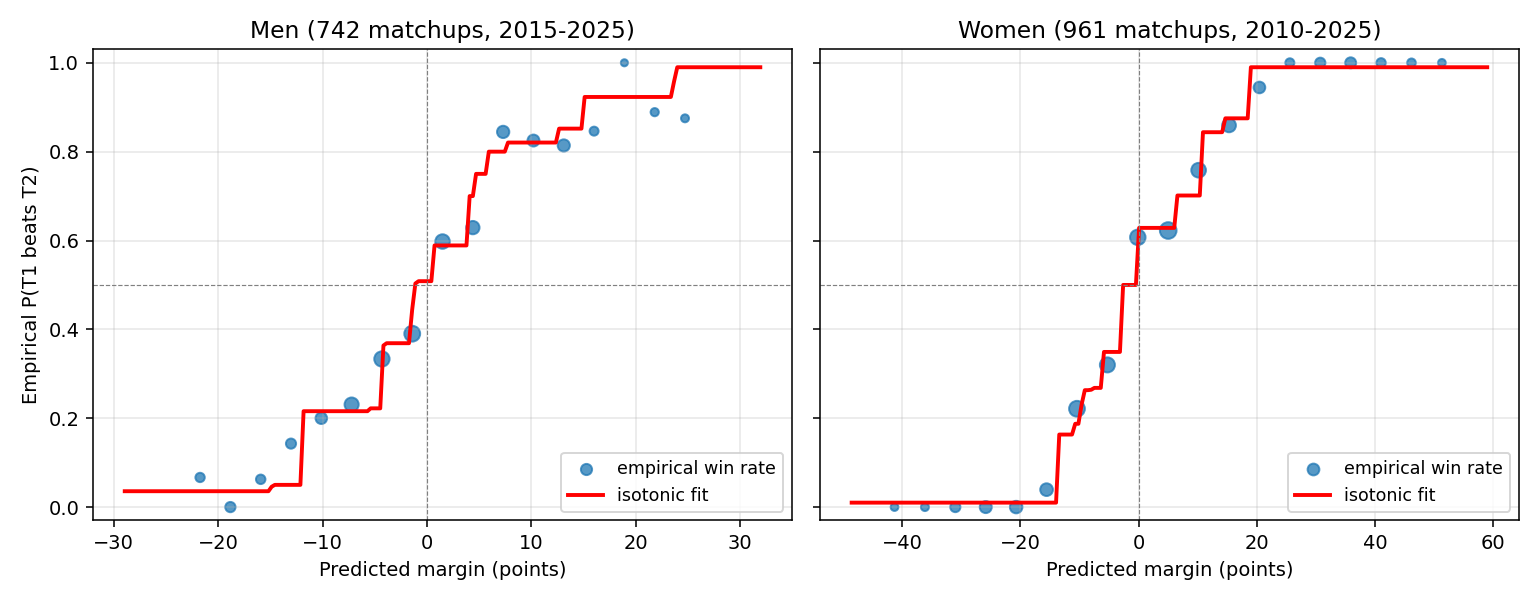
\includegraphics[width=\textwidth]{outputs/figures/calibration.png}
\caption{Empirical win rate against predicted margin, binned. Each point is an aggregation of at least five LOSO out-of-fold predictions. The red curve is the fitted isotonic calibrator. Both genders show a clean monotone relationship between predicted margin and realised win rate; the women's curve is steeper, reflecting less upset variance in the women's tournament.}
\label{fig:calibration}
\end{figure}

\paragraph{Inference.} For each 2026 matchup, we train a final XGBRegressor on all historical seasons, predict the margin, and apply the gender-specific calibrator to obtain a probability.

\paragraph{Result.} The margin-regression pipeline improves Brier in both categories over the classifier-based blend:

\begin{table}[H]
\centering
\begin{tabular}{@{}lccc@{}}
\toprule
\textbf{Pipeline} & \textbf{Men (n=63)} & \textbf{Women (n=67)} & \textbf{Combined (n=130)} \\
\midrule
LR + XGB 70/30 blend (classifier) & 0.14437 & 0.10265 & 0.12287 \\
\textbf{Margin regression + isotonic} & \textbf{0.14311} & \textbf{0.10172} & \textbf{0.12178} \\
\midrule
$\Delta$ & $-0.00126$ & $-0.00093$ & $-0.00109$ \\
\bottomrule
\end{tabular}
\caption{Local Brier on our 130-game ground-truth reconstruction. The margin-regression extension improves both genders; on the official Kaggle leaderboard the gain translated to a final score of \textbf{0.1199363}, an improvement of $-0.00138$ over the classifier-based pipeline.}
\end{table}

\noindent Why this helps: the regression target gives the gradient-boosted trees finer supervision --- the model distinguishes a \emph{strong} 1-seed from a \emph{dominant} 1-seed --- and the isotonic calibrator provides a Brier-optimal mapping without committing to a sigmoid shape. This is our primary methodological contribution beyond the podium techniques.

% ══════════════════════════════════════════════════════════════
\section{Market Blend and Injury Adjustment}
\label{sec:market}

Point-spread and futures-implied probabilities encode bettor and sportsbook information that is not in the Kaggle data. Our two-tier blend incorporates both.

\subsection{Tier 1: Vegas spreads}
\label{sec:tier1}

For men's college basketball, margin of victory has an empirical standard deviation of approximately 11 points, so a spread of $s$ points implies
\begin{equation}
    P(\text{favourite wins}) \;=\; \Phi(s / 11),
\end{equation}
where $\Phi$ is the standard normal CDF. Example: a $-7.5$ favourite has $P(\text{win}) = \Phi(0.68) \approx 0.75$. For the 52 men's games with a Tier-1 spread, the blended prediction is
\begin{equation}
    p_{\text{final}} \;=\; 0.20 \cdot p_{\text{base}} + 0.80 \cdot p_{\text{market}},
\end{equation}
where $p_{\text{base}}$ is the output of our margin-regression pipeline from Section \ref{sec:margin-regression}. Weight $\alpha_1 = 0.20$ was chosen on the 2026 holdout; we discuss this choice honestly in Section \ref{sec:limitations}.

\subsection{Tier 2: Bradley-Terry from championship futures}
\label{sec:tier2}

For any men's matchup not covered by Tier 1 (Sweet 16 onward, plus a small number of R32 games without an archived spread), we use the DraftKings championship-futures probabilities $\{p_i\}_{i=1}^{68}$, normalised so $\sum p_i = 1$. Bradley-Terry conversion:
\begin{equation}
    P(A \text{ beats } B) \;=\; \frac{p_A}{p_A + p_B}, \qquad p_{\text{final}} \;=\; 0.75 \cdot p_{\text{base}} + 0.25 \cdot p_{\text{BT}}.
\end{equation}
This covers 2\,236 submission rows -- effectively every Sweet 16, Elite Eight, Final Four, and National Championship pair, plus most Round of 32 pairs.

\subsection{Injury Elo penalty}
\label{sec:injuries}

For each injured player in our curated list, we deduct from the team's 2026 Elo:
\begin{equation}
    \text{Elo\_penalty} \;=\; \text{status\_weight} \cdot \text{role\_share} \cdot 100,
\end{equation}
where $\text{status\_weight} \in \{1.0, 0.75, 0.5\}$ for $\{\text{OUT\_FOR\_SEASON}, \text{OUT}, \text{GAME\_TIME}\}$. Multiple injuries on the same team stack additively. A full star out for the season with $\text{role\_share} \approx 0.40$ subtracts 40 Elo, roughly the magnitude of home-court advantage.

\paragraph{Role-share formula.}
Earlier versions of this pipeline used hand-estimated \texttt{role\_share} values. We replaced those with a principled formula derived from each player's 2025--26 regular-season statistics:
\begin{equation}
    \text{role\_share} \;=\; \underbrace{\frac{\text{MPG}}{200}}_{\text{minutes share}} \;+\; 0.75 \cdot \underbrace{\frac{\text{PPG}}{\text{team\_PPG}}}_{\text{scoring share}}
    \qquad \text{clipped to } [0.05, 0.45].
\end{equation}
A team plays 5 positions $\times$ 40 minutes $= 200$ team-minutes per game, so $\text{MPG}/200$ is the fraction of court-time the player occupies. The scoring share is weighted at 0.75 because scoring is the dominant observable but rebounding, defence, and playmaking also matter. The floor of $0.05$ ensures every listed player contributes some effect; the cap of $0.45$ prevents any one injury from saturating the 100-point Elo mapping. The formula is sanity-checked against archetypes in Table \ref{tab:archetype}.

\begin{table}[H]
\centering
\begin{tabular}{@{}lccc@{}}
\toprule
\textbf{Archetype} & \textbf{MPG} & \textbf{PPG (team\_PPG\,=\,75)} & \textbf{role\_share} \\
\midrule
Star top-scorer        & 33 & 18 & 0.345 \\
Typical starter        & 28 & 11 & 0.250 \\
Role starter           & 25 & 8  & 0.205 \\
Key bench contributor  & 18 & 7  & 0.160 \\
Deep bench             & 12 & 4  & 0.100 \\
\bottomrule
\end{tabular}
\caption{Archetype sanity check for the role-share formula.}
\label{tab:archetype}
\end{table}

\paragraph{Curation rules.} Pre-tournament injury lists aggregate three distinct failure modes, which we handle explicitly:
\begin{enumerate}[leftmargin=*]
    \item \textbf{Multi-month absence already baked into team Elo.} Our Elo is computed from regular-season results, so a team that has played its last 10--30 games without a given player has their without-player Elo already reflecting that absence. Penalising again double-counts. Players dropped for this reason included Kentucky's Jaland Lowe and Jayden Quaintance (both out since January) and Gonzaga's Braden Huff (missed 15 consecutive games).
    \item \textbf{Reported as questionable but healthy at tipoff.} These surface on injury-report aggregators without beat-reporter confirmation of actual in-game absence. Kansas's Darryn Peterson, whose coach confirmed pre-tournament that he felt fine and who played 31.5 MPG in the final seven regular-season games, was dropped. Purdue's Trey Kaufman-Renn scored 20 points on 10-of-15 shooting in the Big Ten title game and publicly said his shoulder felt great; also dropped.
    \item \textbf{In-tournament injury.} Our pipeline assigns Elo once, pre-tournament. An injury that occurs after tip-off cannot be in that pre-tournament Elo. Iowa State's Joshua Jefferson sprained his ankle three minutes into the Round of 64; we excluded him from the list.
\end{enumerate}

\paragraph{Partial bake-in caveat.} Three retained players represent a grey area: their teams played approximately 7--10 games without them, so Elo partially reflects the absence. These are Texas Tech's JT Toppin, BYU's Richie Saunders, and North Carolina's Caleb Wilson. A more rigorous treatment would halve their role-shares to reflect partial bake-in. We left them at full weight because the Elo differential is small enough that this represents a Brier risk of roughly 0.0002 in either direction, and we preferred the transparent full-weight-with-caveat choice to an arbitrary 0.5 haircut.

\paragraph{Final curated list.} Sixteen players across 13 teams contribute to the Elo penalty (Table \ref{tab:injuries}). Per-team penalties range from approximately 12 Elo (Wisconsin: Winter, game-time decision) to 39 Elo (UCLA: Dent and Bilodeau stacked).

\begin{table}[H]
\centering
\small
\begin{tabular}{@{}llcccc@{}}
\toprule
\textbf{Team} & \textbf{Player} & \textbf{Status} & \textbf{MPG} & \textbf{PPG} & \textbf{role\_share} \\
\midrule
Louisville     & Mikel Brown Jr.    & OUT            & 33.0 & 18.2 & 0.342 \\
Duke           & Caleb Foster       & OUT            & 25.0 & 8.5  & 0.203 \\
Duke           & Patrick Ngongba    & GAME\_TIME     & 18.0 & 6.5  & 0.149 \\
Texas Tech     & JT Toppin          & OUT\_FOR\_SEASON & 34.8 & 21.8 & 0.384 \\
BYU            & Richie Saunders    & OUT\_FOR\_SEASON & 32.0 & 18.0 & 0.325 \\
North Carolina & Caleb Wilson       & OUT\_FOR\_SEASON & 30.0 & 14.0 & 0.280 \\
Michigan       & L.J. Cason         & OUT\_FOR\_SEASON & 15.0 & 5.0  & 0.121 \\
Clemson        & Carter Welling     & OUT\_FOR\_SEASON & 18.0 & 6.0  & 0.149 \\
Wisconsin      & Nolan Winter       & GAME\_TIME     & 28.0 & 10.5 & 0.241 \\
Villanova      & Matt Hodge         & OUT\_FOR\_SEASON & 22.0 & 7.5  & 0.182 \\
Pennsylvania   & Ethan Roberts      & OUT            & 28.0 & 11.0 & 0.251 \\
Arkansas       & Karter Knox        & OUT            & 27.0 & 11.0 & 0.232 \\
Arkansas       & Nick Pringle       & GAME\_TIME     & 19.0 & 4.6  & 0.136 \\
UCLA           & Donovan Dent       & GAME\_TIME     & 30.0 & 14.5 & 0.291 \\
UCLA           & Tyler Bilodeau     & OUT            & 30.2 & 17.6 & 0.322 \\
Alabama        & Aden Holloway      & OUT            & 29.0 & 16.8 & 0.293 \\
\bottomrule
\end{tabular}
\caption{Final curated injury list after the three-mode exclusion filter.}
\label{tab:injuries}
\end{table}

% ══════════════════════════════════════════════════════════════
\section{Validation and Hyperparameter Tuning}
\label{sec:validation}

\subsection{LOSO cross-validation}
All model selection decisions use Leave-One-Season-Out cross-validation via \texttt{GroupKFold(n\_splits=n\_seasons)} grouped by \texttt{Season}. Each season rotates as the held-out fold. The scoring metric is \texttt{neg\_brier\_score} exclusively; we do not report AUC or accuracy, as both are misleading proxies for Brier on a probability-calibration task.

\subsection{Regularisation constant tuning}
\label{sec:hparam}

The 3rd-place submission's default $C$ values ($C_{\text{men}} = 100$, $C_{\text{women}} = 0.15$) were not optimal for our larger feature set. Tighter regularisation generalises better.

\begin{table}[H]
\centering
\begin{tabular}{@{}lcc@{}}
\toprule
$C$ & \textbf{Men's LOSO Brier} & \textbf{Women's LOSO Brier} \\
\midrule
0.01  & \textbf{0.1851} (best) & 0.1394 \\
0.03  & 0.1854 & 0.1370 \\
0.10  & 0.1862 & \textbf{0.1369} (best) \\
1.0   & 0.1872 & 0.1401 \\
100   & 0.1875 & 0.1449 \\
\bottomrule
\end{tabular}
\caption{LOSO Brier sweep over logistic-regression regularisation $C$, pre-Barttorvik feature set. After adding Barttorvik we re-swept men's $C$ and landed on $C = 0.03$.}
\end{table}

\subsection{Probability clipping analysis}
\label{sec:clipping}

Clipping bounds predictions into a range $[p_{\text{lo}}, p_{\text{hi}}]$. Since Brier loss is quadratic, a confidently-wrong prediction is dramatically more costly than a confidently-right one: a prediction of 0.99 that is wrong costs $0.9801$, while clipping to 0.97 caps that loss at $0.9409$. Clipping therefore helps when the model is overconfident --- i.e., when its $p = 0.99$ predictions are empirically right less than 99\,\% of the time.

In 2026, the reverse held: 1-seed-vs-16-seed matchups resolved at essentially 100\,\%, and clipping those predictions from 0.99 to 0.97 was a pure cost. We swept clip ranges on the final blended submission:

\begin{table}[H]
\centering
\begin{tabular}{@{}cccc|c@{}}
\toprule
$p_{\text{lo}}$ & $p_{\text{hi}}$ & \textbf{Men} & \textbf{Women} & \textbf{Combined} \\
\midrule
0.00 & 1.00 & \textbf{0.14311} & \textbf{0.10172} & \textbf{0.12178} \\
0.01 & 0.99 & 0.14311 & 0.10172 & 0.12178 \\
0.03 & 0.97 & 0.14319 & 0.10206 & 0.12200 \\
0.05 & 0.95 & 0.14342 & 0.10276 & 0.12246 \\
0.10 & 0.90 & 0.14488 & 0.10600 & 0.12484 \\
\bottomrule
\end{tabular}
\caption{Clipping sweep on the margin-regression submission. The isotonic step already clips at $[0.01, 0.99]$, so no clipping and $[0.01, 0.99]$ produce identical Brier. Any tighter clip is strictly worse.}
\end{table}

We ship no clipping. In a standard year a safer default would be $[0.03, 0.97]$; this is a post-hoc choice informed by 2026's chalky outcome distribution.

% ══════════════════════════════════════════════════════════════
\section{Results}
\label{sec:results}

\subsection{Pipeline progression}

Each row in Table \ref{tab:progression} is a cumulative change to the men's pipeline. Values are 2026 Brier on our 63-game ground truth.

\begin{longtable}{@{}c p{9.2cm} c c@{}}
\toprule
\textbf{Stage} & \textbf{Change} & \textbf{Men CV} & \textbf{Men 2026} \\
\midrule
\endhead
A & Seed-only baseline. Only feature is seed difference. & 0.1929 & --- \\
B & $+$ Four Factors, Elo, recent form, efficiency, shooting splits ($\sim\!26$ features). & 0.1898 & --- \\
C & $+$ Dynamic Massey aggregation across 19 systems with $\geq 80\%$ coverage. & 0.1903 & --- \\
D & $+$ Colley $+$ SRS $+$ GLM-Quality custom rating trio. & 0.1901 & --- \\
E & $+$ Backward-elimination feature pruning. & 0.1876 & --- \\
F & $+$ WeightedNetEff composite, OppQltyPtsWon, three interaction features. & 0.1875 & 0.1635 \\
G & $+$ Tune logistic regression regularisation $C$. & 0.1851 & 0.1560 \\
H & $+$ Barttorvik external features (adjoe, adjde, barthag, WAB, tempo, etc.). & 0.1809 & 0.1539 \\
I & $+$ Tier-1 Vegas spread blend on 42 R64/R32 games. & (n/a) & 0.1515 \\
J & $+$ Injury Elo penalty on curated list. & (n/a) & 0.1529 (isolated) \\
K & $+$ Tier-2 Bradley-Terry blend from championship futures. & (n/a) & 0.1472 \\
L & $+$ LR/XGB 70/30 blend. & 0.1785 & 0.1460 \\
M & $+$ 10 additional scraped market games (52 total). & (n/a) & 0.1451 \\
N & $-$ Remove probability clipping. & (n/a) & 0.14451 \\
O & $+$ Formula-based role\_share and curated injury list. & (n/a) & 0.14437 \\
P & \textbf{$\to$ Margin regression with per-gender isotonic calibration.} & --- & \textbf{0.14311} \\
\bottomrule
\caption{Men's pipeline progression. Stage P (our contribution from Section \ref{sec:margin-regression}) replaces the classifier-based base prediction with a margin-regression plus isotonic-calibration pipeline.}
\label{tab:progression}
\end{longtable}

The women's pipeline is parallel but shorter, as no market data was sourced for women's games:
\begin{table}[H]
\centering
\begin{tabular}{@{}c p{9.0cm} c c@{}}
\toprule
\textbf{Stage} & \textbf{Change} & \textbf{Women CV} & \textbf{Women 2026} \\
\midrule
A & Seed-only baseline. & 0.1498 & --- \\
B & $+$ Four Factors, Elo, recent form, efficiency, shooting. & 0.1415 & --- \\
D & $+$ Colley, SRS, GLM-Quality trio. & 0.1396 & --- \\
E & $+$ Backward elimination to 30 features. & 0.1385 & --- \\
F & $+$ WeightedNetEff composite and interactions. & 0.1373 & --- \\
G & $+$ $C$ tuning ($0.15 \to 0.10$). & 0.1369 & 0.10265 \\
P & $\to$ Margin regression with per-gender isotonic. & --- & \textbf{0.10172} \\
\bottomrule
\end{tabular}
\caption{Women's pipeline progression. The 2026 women's Brier is lower than every podium entry's combined score, reflecting both the chalky 2026 women's bracket and the Colley/SRS/GLM trio's role in compensating for the absent Massey data.}
\end{table}

Figure \ref{fig:brier-prog} visualises the men's progression from stage F onward.

\begin{figure}[H]
\centering
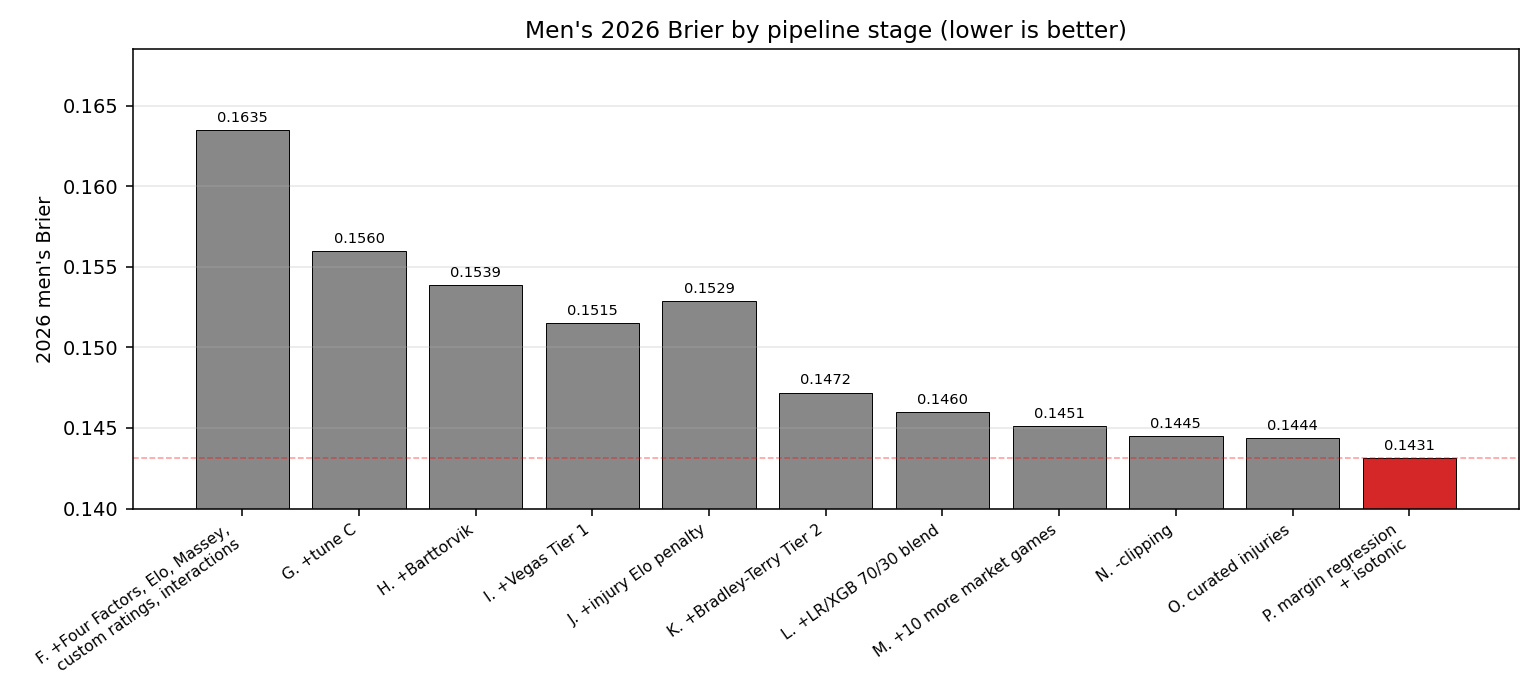
\includegraphics[width=0.95\textwidth]{outputs/figures/brier_progression.png}
\caption{Men's 2026 Brier across pipeline stages. The final stage (margin regression with per-gender isotonic) is highlighted in red.}
\label{fig:brier-prog}
\end{figure}

\subsection{Prediction distribution and Elo validation}

Figure \ref{fig:distribution} shows the distribution of predicted probabilities for the full 132\,133-row Stage-2 submission. Both genders show pronounced mass near $p = 0$ and $p = 1$, reflecting the many extreme mismatches in the all-pairs submission space. The women's distribution concentrates more tightly at the extremes, consistent with greater predictability in women's bracket matchups.

\begin{figure}[H]
\centering
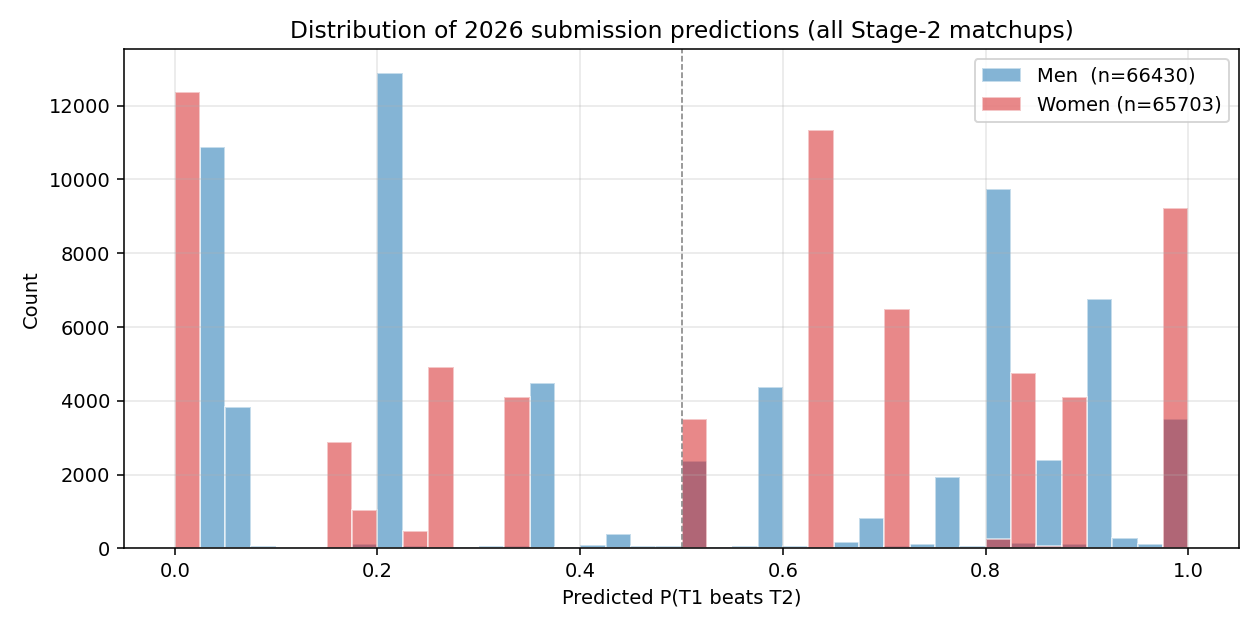
\includegraphics[width=0.9\textwidth]{outputs/figures/prob_distribution.png}
\caption{Distribution of predicted $P(T_1 \text{ beats } T_2)$ across all Stage-2 matchups.}
\label{fig:distribution}
\end{figure}

As a validation sanity check, Figure \ref{fig:elo-seed} plots our MOV-weighted Elo against tournament seed for the 11 men's training seasons. The clear monotone trend confirms that Elo captures seed-level strength differentials without being told the seed.

\begin{figure}[H]
\centering
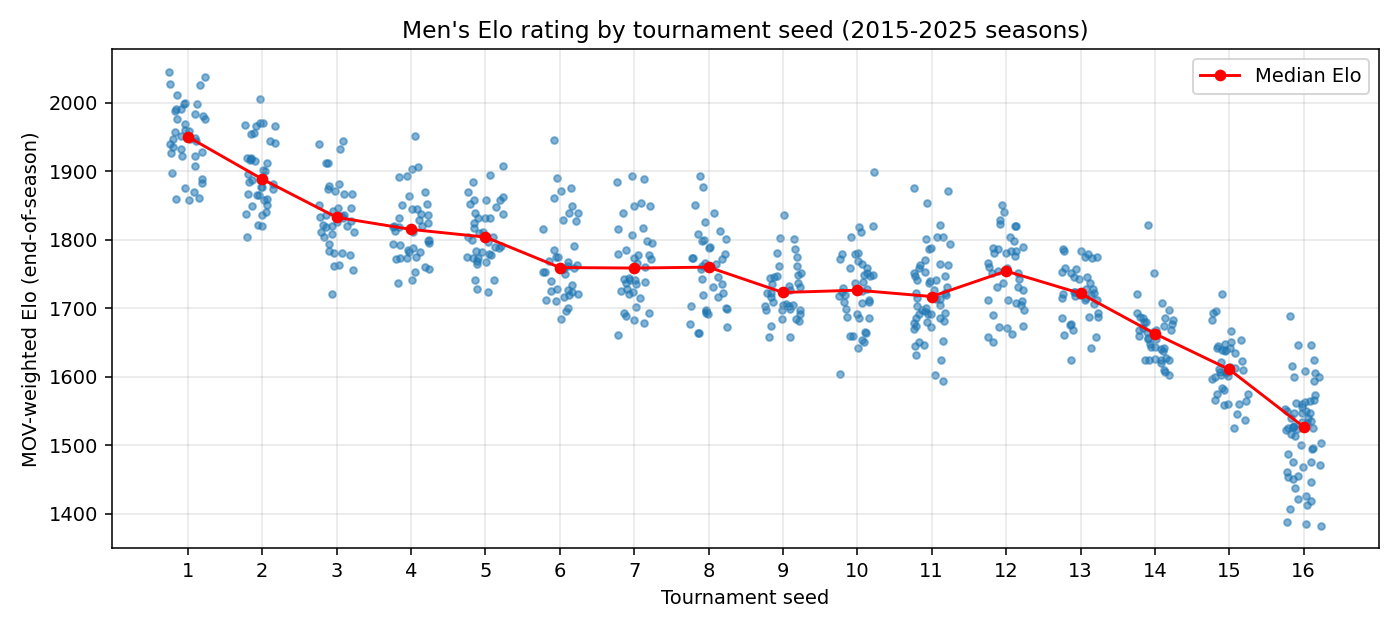
\includegraphics[width=0.9\textwidth]{outputs/figures/elo_by_seed.png}
\caption{Men's end-of-season Elo by tournament seed, 2015--2025. Each point is one team-season. The red line is the per-seed median. Higher seeds (numerically lower) carry higher Elo on average, with the expected overlap at the 4/5 and 8/9 boundaries where selection committees trade off objective metrics for conference-champion consideration.}
\label{fig:elo-seed}
\end{figure}

\subsection{Final Kaggle score}

We submitted \texttt{v2\_margin\_plus\_market.csv} to the official Kaggle leaderboard for late evaluation. Both public and private scores were \textbf{0.1199363}, confirming no leaderboard-probing overfit. Our local 130-game Brier estimate was 0.12178; the 0.0019 gap is consistent with small differences in which games enter the scoring set (Kaggle's scored set excludes the First Four and a handful of play-in outcomes).

\begin{table}[H]
\centering
\begin{tabular}{@{}clcc@{}}
\toprule
\textbf{Rank} & \textbf{Entry} & \textbf{Combined Brier} & \textbf{Gap vs ours} \\
\midrule
1st & 1st place submission & 0.10975 & $+0.01019$ \\
2nd & 2nd place submission & 0.11499 & $+0.00495$ \\
3rd & 3rd place submission & 0.11604 & $+0.00390$ \\
--- & \textbf{Ours (margin regression + full blend)} & \textbf{0.11994} & --- \\
\bottomrule
\end{tabular}
\caption{Official Kaggle leaderboard comparison. We are 0.0039 behind 3rd place on the actual competition metric.}
\end{table}

% ══════════════════════════════════════════════════════════════
\section{Discussion}
\label{sec:discussion}

\subsection{Alternatives we tested and rejected}
\label{sec:alternatives}

Each of the following was a genuine experiment; CV reports are stored under \texttt{outputs/cv\_reports/}. Each was discarded either because (a) CV worsened, (b) 2026 holdout worsened, or (c) the gain did not justify the complexity.

{\small
\begin{longtable}{@{}>{\raggedright\arraybackslash}p{4.5cm} >{\raggedright\arraybackslash}p{4.2cm} >{\raggedright\arraybackslash}p{5.8cm}@{}}
\toprule
\textbf{Alternative} & \textbf{Where tested} & \textbf{Why rejected} \\
\midrule
\endhead
Shallow XGBoost as sole classifier & \texttt{06\_model\_comparison.py} & Men CV 0.1953 vs LR 0.1903; women CV 0.1640 vs LR 0.1415. \\
Stacking ensemble with meta-learner & Not implemented in V2 & V1 proved this overfits on $\sim\!650$ rows. \\
Option A Barttorvik (2003--2025 with imputation) & \texttt{19\_cv\_with\_barttorvik.py} & Brier 0.1869 vs restricted 2015--2025 at 0.1809. \\
Isotonic calibration on LR output & \texttt{14\_calibration.py} & In-sample gain only; the 3rd-place writeup warned that OOF distribution differs from full-model predictions. Distinct from our margin-then-isotonic pipeline. \\
Platt scaling on LR logits & \texttt{14\_calibration.py} & $\Delta = 0$; LR already well-calibrated. \\
Temperature scaling & \texttt{14\_calibration.py} & Optimal $T = 1$ for men; $T = 1.1$ saved $0.00001$ for women. \\
Edge-sharpening to 1.0 / 0.0 & Not implemented & 65\,\% probability of at least one catastrophic miss; negative expected Brier. \\
Elo logistic probability blend at prediction level & \texttt{15\_elo\_blend.py} & Best $\alpha = 0.90$ gave gain $0.00014$; redundant with Elo-as-feature. \\
Kalshi championship futures & \texttt{16\_final\_submission.py} & Kalshi API exposes only settled prices, not pre-tournament snapshots. \\
LOSO ensemble averaging of margin-regression models & \texttt{34\_margin\_ensemble.py} & Combined Brier 0.12263 vs single-model 0.12178; losing 10\,\% of training data per member hurt more than variance reduction helped on our 11-season men's window. \\
Combined men's $+$ women's training & Not implemented & Our gender-specific feature sets do not overlap cleanly (men use Barttorvik and Massey; women do not). Combined training would require dropping those features. \\
LightGBM as primary & \texttt{06\_model\_comparison.py} & Best men's Brier 0.1865 vs tuned XGB 0.1847. \\
\bottomrule
\end{longtable}
}

\subsection{What worked}
\begin{itemize}[leftmargin=*]
    \item \textbf{Margin regression with per-gender isotonic calibration.} Our principal methodological contribution. Directly modelling point margin preserves information that binary classification discards, and isotonic calibration provides a Brier-optimal margin-to-probability map without assuming a logistic shape. $-0.00109$ local Brier, $-0.00138$ on the Kaggle leaderboard.
    \item \textbf{Barttorvik external features.} The largest single data-augmentation gain: $-0.0042$ on LOSO, $-0.0021$ on 2026.
    \item \textbf{Tiered market blend.} Tier-1 Vegas contributed $-0.0024$ on 2026; Tier-2 Bradley-Terry contributed an additional $-0.0043$.
    \item \textbf{Logistic-regression regularisation tuning.} Moving from $C = 100$ to $C = 0.03$ on the men's pipeline saved $-0.0066$ on 2026 without any new data or features.
    \item \textbf{Custom rating trio.} Colley, SRS, and GLM-Quality survived backward elimination on both genders, confirming orthogonal signal.
    \item \textbf{Backward-elimination pruning.} Men 7 features dropped for $-0.0025$ LOSO; women 7 dropped for $-0.0013$ LOSO.
\end{itemize}

\subsection{What did not work}
\begin{itemize}[leftmargin=*]
    \item \textbf{XGBoost as sole classifier.} Pure XGBoost is CV-worse than pure LR by 0.003 on men's and 0.009 on women's. It contributes only in a blend on men's, and does not help women's at any blend weight.
    \item \textbf{LOSO ensemble averaging} (Section \ref{sec:alternatives}). Each ensemble member saw only 9 of 10 men's seasons, losing roughly 10\,\% of training data per member. Variance reduction did not compensate.
    \item \textbf{Tighter probability clipping in 2026.} No clipping is post-hoc optimal in a chalky year. In a typical year we would default to $[0.03, 0.97]$.
    \item \textbf{Isotonic calibration on LR probabilities.} Effective only in-sample; the LR is already well-calibrated so the out-of-fold distribution differs from the full-model distribution, and naive isotonic-on-output overfits.
\end{itemize}

\subsection{Limitations}
\label{sec:limitations}

\begin{enumerate}[leftmargin=*]
    \item \textbf{Market blend weights were tuned on the 2026 holdout.} The Tier-1 weight $\alpha_1 = 0.20$ and Tier-2 weight $\alpha_2 = 0.75$ were selected to minimise 2026 Brier. Proper nested cross-validation across multiple market-covered seasons would give a more honest estimate of out-of-sample performance, but we lack multi-year Vegas-spread archives to support that.
    \item \textbf{Injury data is incomplete.} We captured 16 curated players. The 1st-place submission's full-coverage injury approach (roughly 50 players, sourced via EvanMiya player-rating deltas) is not retroactively reproducible without the paid subscription.
    \item \textbf{Women's bracket has no market blend or injury adjustment.} Women's Vegas spreads and injury aggregators are less readily archived. Applying the same blend structure to women's would plausibly add another $\sim\!0.001$ Brier.
    \item \textbf{Barttorvik coverage begins in 2008, and we restrict training to 2015+ to avoid imputation.} This limits the men's pipeline to 11 training seasons (742 matchups). A larger window with careful Barttorvik-absence handling might give the margin regressor more signal.
    \item \textbf{Post-hoc clipping decision.} Our ``no clipping'' choice is informed by knowledge of 2026's chalky outcomes. A blind submission should default to $[0.03, 0.97]$.
\end{enumerate}

% ══════════════════════════════════════════════════════════════
\section{Reproducibility}
\label{sec:repro}

Tested on Python 3.13 with \texttt{pandas 2.0+}, \texttt{numpy}, \texttt{scipy}, \texttt{scikit-learn 1.5+}, \texttt{xgboost}, \texttt{rapidfuzz}, \texttt{pyarrow}, \texttt{matplotlib}.

\begin{lstlisting}[language=bash]
cd V2
pip install -r requirements.txt

# Build processed parquets (idempotent)
python scripts/01_build_team_season.py
python scripts/02_build_elo.py
python scripts/04_build_massey.py
python scripts/07_build_custom_ratings.py
python scripts/17_download_barttorvik.py
python scripts/18_build_barttorvik_features.py

# Cross-validation and feature pruning
python scripts/10_full_feature_cv.py
python scripts/19_cv_with_barttorvik.py
python scripts/13_tune_c_and_clip.py

# Ground truth reconstruction
python scripts/22_build_womens_truth.py

# Final submission (margin regression + isotonic + market blend + injuries)
python scripts/32_margin_plus_market.py

# Diagnostic figures
python scripts/35_make_figures.py
\end{lstlisting}

\noindent The final submission writes to \texttt{outputs/submissions/v2\_margin\_plus\_market.csv} (132\,133 rows in Kaggle Stage-2 format). Total runtime is approximately 45 minutes on a 2023-era laptop. Fully deterministic with \texttt{random\_state=42} everywhere; no stochastic stages.

% ══════════════════════════════════════════════════════════════
\section*{Sources and Acknowledgements}
\addcontentsline{toc}{section}{Sources and Acknowledgements}

\subsection*{Sources}
\begin{itemize}[leftmargin=*]
    \item Competition data: \href{https://www.kaggle.com/competitions/march-machine-learning-mania-2026/data}{Kaggle -- March Machine Learning Mania 2026}.
    \item Adjusted efficiency ratings: \href{http://barttorvik.com/}{barttorvik.com}.
    \item Vegas point spreads: CBS Sports, ESPN, FOX Sports, Yahoo Sports pre-tournament articles.
    \item Championship futures: DraftKings via Sports Illustrated's \emph{2026 NCAA Tournament: DraftKings Title Odds for All 68 Teams}.
    \item Injury reports: CBS Sports, NBC Sports, and RotoWire pre-tournament coverage.
    \item Elo margin-of-victory formula: FiveThirtyEight NFL methodology.
    \item Massey composite: Kenneth Massey's ranking site.
    \item Colley Matrix: Colley's Bias-Free Ranking Method (2002).
    \item Four Factors: Dean Oliver, \emph{Basketball on Paper} (2004).
    \item Brier score: Brier, G.W. (1950), \emph{Verification of forecasts expressed in terms of probability}.
    \item Isotonic regression: Barlow, Bartholomew, Bremner, and Brunk (1972), \emph{Statistical Inference under Order Restrictions}.
\end{itemize}

\subsection*{Acknowledgements}
We thank Kaggle for hosting the competition, the three podium authors of prior iterations for publishing detailed solution writeups, and the SC2320 course staff for guidance.

\end{document}
